\chapter{The Constrained Optimal Top-$m$ Allocation}\label{chapter:optimal}
%What does it mean to be optimal?
Analogously to \ref{subsection:optimal_allocation}, we define the optimal
top-$m$ allocation by its convergence rate of the posterior mass put on
parameters reflecting the true top-$m$ arms $\Pi_n(\Theta_{S^*})$. This, too can
be thought of as a thought experiment of convincing an adversary by relying on
knowledge of the true means.  Moreover, just as in Russo's top-1 case, the
algorithm we will propose introduces a constraint. We will also put the optimal
allocation under that constraint with the idea being that this is but a
hyperparameter that can be optimized over. In other words: the best
unconstrained allocation is the best constrained allocation with optimal
hyperparameter.

In \Cref{section:optimal_statements} we first introduce some of Russo's results
that also apply in our scenario. Then we will introduce some general properties,
followed by a complete characterization of the optimal allocation. Moreover, we
will show an example of a concrete optimal allocation in
\Cref{section:concrete_optimal_allocation}. Proofs of the statements from
\Cref{section:optimal_statements} are provided in \Cref{section:optimal_proofs}.
We finish the chapter with \Cref{section:optimality_sufficient_condition}, a
presenting a condition on adaptive allocations, which is sufficient to show
convergence to the optimal allocation.

Overall we hope to convince the reader that the characterization results
portrayed in this chapter make for a natural generalization of Russo's top-1
case. In the top-1 case, Russo implied comparing the best arm $l^*$ to a
suboptimal arm in order to identify the one it is hardest to distinguish from
it. Our guiding theme, on the other hand, will be to compare the a pairs of
optimal and suboptimal arms in order to find to the pair that is the hardest to
distinguish. Note that again, distinction revolves around two factors: the
frequency with which an arm has been sampled, $\bar{\psi}_{n, l}$, as well as
the proximity of its true mean, i.e. comparing $\theta^*_l$.

Throughout this whole chapter we will assume that every true mean is unique,
i.e.
\begin{align}
  \forall l_1, l_2 \in [k]: l_1 \neq l_2 \Rightarrow \theta^*_{l_1} \neq
      \theta^*_{l_2}
\end{align}
and as previously mentioned that the underlying true means follow distributions
belonging to the family of exponential distributions.
%%%%%%
% Statements
%How can C be interpreted?
%How does this tie in with Chernoff's statements?
%How does this compare to the top-1 case?
%What's an example of an optimal allocation?
%How would those statements look like without the constraint?
%%%%%

\section{Characterization statements}\label{section:optimal_statements}
Russo proves a proposition about the posterior convergence rate of general
parameter sets $\tilde{\Theta}$.

\begin{proposition}[Russo: Proposition 5]\label{proposition:prop5}
  For any open set $\tilde{\Theta} \subset \Theta$ and average allocation
  $\bar{\psi}_n$
  \begin{align}
    \Pi_n(\tilde{\Theta}) \deq \exp\{-n \inf_{\theta \in
        \tilde{\Theta}} \sum_{l \in [k]} \bar{\psi}_{n, l} d(\theta^*_l ||
        \theta_l)\}
  \end{align}
\end{proposition}

This proposition already sets the tone by expressing that the posterior of a set
depends on a property of a single contained element $\theta$. The property in
question is how hard it is to distinguish $\theta$ from the truth $\theta^*$. As
we've stressed, the optimal allocation $\psi^*$ is non-adaptive and fixed over
time. Thereby the average allocation $\bar{\psi}^*$ corresponds to
$\psi^*$.

As mentioned before, we seek to analyze how fast $\Pi_n(\Theta_{S^*})$ converges
to 1. Clearly we have $\Theta_{S^*} = \Theta - \Theta_{S^*}^c$. Hence instead of
analyzing the rate of convergence of $\Pi_n(\Theta_{S^*})$ to 1, we can analyze
the rate of convergence of $\Pi(\Theta_{S^*}^c)$ to 0.

Instead of analyzing $\Pi_n(\Theta_{S^*}^c)$ directly, we express it via
$\Theta_{m, l}$ and its relaxation $\bar{\Theta}_i$. Intuitively,
$\bar{\Theta}_i$ is the set of parameters under which $i$ proves that $S^*$ is
not optimal.
\begin{align}
  \bar{\Theta}_i &= \{ \theta \in \Theta | \text{top-}m(\theta, S^* \cup
      \{i\}) \neq S^*\}
\end{align}
Observe that we have $\bar{\Theta}_i \supsetneq \Theta_{m, i}$. Moreover we
present a useful relationship between $\Theta_{S^*}^c$ and $\bar{\Theta}_i$:
\begin{lemma}\label{lemma:set_relation_S*_i}
  \begin{align}
    \Theta_{S^*}^c = \bigcup_{i \notin S^*} \bar{\Theta}_i = \Theta -
        \bigcap_{j \in S^*} \Theta_{m, j}
  \end{align}
\end{lemma}
Leveraging this relationship of the sets allows us to bridge the gap between the
posterior of $\Theta_{S^*}^c$ and the posterior of individual sets
$\bar{\Theta}_i$. Note the transition from a union of sets to a minimum over
sets permitted by the usage of the $\deq$ relation, as shown in
\Cref{lemma:posterior_S*_i}.
\begin{lemma}
  \label{lemma:posterior_S*_i} If $\alpha_{n, S^*} \rightarrow 1$, then
  \begin{align}
    \Pi_n(\Theta_{S^*}^c) \deq \max_{i \notin S^*} \Pi_n(\bar{\Theta}_i) \deq 1
        - \min_{j \in S^*} \Pi_n(\Theta_{m, j})
  \end{align}
\end{lemma}

Plugging $\bar{\Theta}_i$ into \Cref{proposition:prop5} leaves us with a sum of
KL divergences. We seek to simplify this sum to individual terms just after
defining:
\begin{align}
  C_{j, i}(p_1, p_2) &= \min_{x \in \mathbb{R}} p_1 d(\theta^*_{j} || x) + p_2
      d(\theta_{i}^* ||x) \label{eq:C}
\end{align}
Usually we will encounter $C_{j, i}$ with its firs argument being the
measurement plan for arm $j$, $\psi_j$ and its second argument being the
measurement plan for arm $i$, $\psi_i$.
%TODO: Talk about player scenario?

In particular, $C_{j, i}$ can be thought of as evidence that $j$ is distinct
from $i$. Quite naturally, we want this evidence to be as large as possible for
every pair $(j, i) \in S^* \times {S^*}^c$.

\begin{lemma}\label{lemma:kl_to_C}
  For any $i \notin S^*$ and any allocation $\psi$,
  \begin{align}
    \min_{\theta \in \bar{\Theta}_i} \sum_{l \in [k]}\psi_l
        d(\theta^*_l||\theta_l) = \min_{j \in S^*} C_{j, i}(\psi_j, \psi_i)
  \end{align}
\end{lemma}

Intuitively, this lemma tells us that for parameters in $\Bar{\Theta}_i$ the
weighted sum of KL divergences can be by simplified to only two arms. One of
those arms will be $i$. The other has arm to stem from the true set of arms
$S^*$ in order to satisfy $\Bar{\Theta}_i$'s requirement of 'disproving' $S^*$.
This arm $j \in S^*$ is chosen as to seem the 'least distinctive' from $i$.
Distinction is made up of two aspects, as seen in the definition of $C_{j, i}$
in \eqref{eq:C}: how much this arm $j$ is sampled, i.e. $\psi_j$, and how
different its true mean $\theta^*_j$ is from the true mean $\theta^*_i$ of $i$.
The latter difference is captured by the KL divergence between both arms and a
minimal $x$, individually.

We can apply those statements to the quantity we care about: the mass the
posterior puts on the complement of parameters reflecting the true top-$m$ arms,
$\Theta_{S^*}^c$.

For a given fixed allocation $\psi$, we have:
\begin{align}
  \Pi_n(\Theta_{S^*}^c) &\deq \max_{i \notin S^*}\Pi_n(\bar{\Theta}_i) \text{ (\Cref{lemma:posterior_S*_i})}\\
    &\deq \max_{i \notin S^*} \exp\{-n\inf_{\theta \in \bar{\Theta}_i} \sum_{l
        \in [k]} \psi_{n, l} d(\theta^*_l || \theta_l)\} \text{
        (\Cref{proposition:prop5})} \\
    &= \max_{i \notin S^*} \exp\{-n \min_{j \in S^*} C_{j, i}(\bar{\psi_j},
        \bar{\psi_i})\} \text{ (\Cref{lemma:kl_to_C})} \\
    &= \exp\{-n \min_{i \notin S^*}\min_{j \in S^*} C_{j, i}(\bar{\psi_j},
        \bar{\psi_i})\} \label{eq:posterior}
\end{align}
In other words, the rate at which the posterior converges to the truth with
increasing number of samples is defined by the pair of optimal and suboptimal
arms for which the least evidence exists.

As we've described, the optimal allocation $\psi^{\frac{1}{2}*}$ is the one
which makes the quantity from \Cref{eq:posterior} as small as possible. We have:
\begin{align}
  \psi^{\frac{1}{2}*} &= \argmin_{\psi} \exp\{-n \min_{i \notin S^*}\min_{j \in
      S^*} C_{j, i}(\psi_j, \psi_i)\} \\
    &= \argmax_{\psi} \min_{i \notin S^*}\min_{j \in S^*} C_{j, i}(\psi_j,
        \psi_i) \label{eq:psi^*}
\end{align}
For the sake of convenience we define the optimal exponent:
\begin{align}
  \Gamma^* = \max_{\psi} \min_{i \notin S^*}\min_{j \in S^*} C_{j, i}(\psi_j,
      \psi_i) \label{eq:gamma^*}
\end{align}

\paragraph{An Optimal Constrained Allocation}

Our proposed algorithm will always allocate $\frac{1}{2}$ of its samples to arms
in $S^*$ in the long run. As a consequence it may not attain the overall optimal
exponent without hyperparameter tuning. Hence we consider a modified,
constrained setting under which the algorithm performs optimally. By adapting
\eqref{eq:psi^*} and \eqref{eq:gamma^*} we obtain:
\begin{align}
  \psi^{\frac{1}{2}*} &= \argmax_{\psi: \psi_{S^*}=\frac{1}{2}} \min_{i \notin
      S^*}\min_{j \in S^*} C_{j, i}(\psi_j, \psi_i)
      \label{eq:constrained_optimal_psi}\\
  \Gamma^{\frac{1}{2}*} &= \max_{\psi, \psi_{S^*} = \frac{1}{2}} \min_{i \notin
      S^*} \min_{j \in S^*} C_{j, i}(\psi_j, \psi_i)
      \label{eq:constrained_optimal_gamma}
\end{align}
Hence we have established the optimal constrained rate of convergence
$\Gamma^{\frac{1}{2}*}$ of the optimal constrained allocation
$\psi^{\frac{1}{2}*}$ by making a link to the minimization over $C_{j, i}$ . We
seek to further characterize $\psi^{\frac{1}{2}*}$ by relying on the same maxim
as in Russo's scenario: we expect the measurement plan to collect \emph{equal
evidence}, not \emph{equal measurement} for every arm. Hence in
\Cref{proposition:characterization} we will show that the optimal measurement
plan will fulfill \Cref{eq:condition_C}. Before doing so, we set the stage by
enunciating three properties of $C_{j, i}$: concavity, existence of a unique
solution $x$ and strict monotonicity.

\begin{lemma}\label{lemma:C_concave}
  Each $\min_{j \in S^*} C_{j, i}(\psi_j, \psi_i)$ is a concave function.
\end{lemma}

\begin{lemma}\label{lemma:C_unique_solution}
  Assume $A'(\theta)$ to be the mean observation under $\theta$. Given a $j \in
  S^*$, the solution to the minimization problem \eqref{eq:C} in $x$ is
  $\bar{\theta} \in \mathbb{R}$, satisfying:
  \begin{align}
    A'(\bar{\theta}) = \frac{\psi_j A'(\theta_j^*) + \psi_i
        A'(\theta_i^*)}{\psi_j + \psi_i}
  \end{align}
  Therefore
  \begin{align}
    C_{j, i}(\psi_j, \psi_i) = \psi_j d(\theta^*_j || \bar{\theta}) + \psi_i
        d(\theta^*_i || \bar{\theta})
  \end{align}
\end{lemma}

\begin{lemma}\label{lemma:C_strictly_increasing}
  For fixed $i \notin S^*$ and $j \in S^*$, $C_{j, i}$ is strictly increasing
  in both of its arguments.
\end{lemma}

\begin{proposition}\label{proposition:characterization}
  The solution to the optimization problem \ref{eq:constrained_optimal_psi} is
  the allocation $\psi^{\frac{1}{2}*}$, which is unique and satisfies
  \begin{align}
    \forall j_1, j_2 \in S^*, \forall i_1, i_2 \notin S^*:
    C_{j, i}(\psi^{\frac{1}{2}*}_{j_1}, \psi^{\frac{1}{2}*}_{i_1})
    = C_{j, i}(\psi^{\frac{1}{2}*}_{j_2}, \psi^{\frac{1}{2}*}_{i_2})
    \label{eq:condition_C}
  \end{align}
  If $\psi_n = \psi^{\frac{1}{2}*}$ for all $n$, then
  \[\Pi_n(\Theta_{S^*}^c) \deq \exp \{-n\Gamma^*_{\frac{1}{2}}\}.\]
  Moreover, under any other adaptive allocation rule, if $\bar{\psi}_{n, S^*}
  \rightarrow \frac{1}{2}$ then
  \[\lim_{n \rightarrow \infty} \sup - \frac{1}{n} \log \Pi_n(\Theta^c_{S^*})
      \leq \Gamma^*_{\frac{1}{2}}\]
  almost surely.
\end{proposition}

The attentive reader might have noticed that we started off with relations between $\Theta_{S^*}$ and both suboptimal arms $i$ and optimal $j$, such as in \Cref{lemma:set_relation_S*_i} and \Cref{lemma:posterior_S*_i}. We stopped doing so in \Cref{lemma:kl_to_C} and proceeded to rely on $i$. We are confident in saying that the same results could have been reached by focusing on $j$, through symmetry.

\section{A concrete optimal allocation}
    \label{section:concrete_optimal_allocation}
For the sake of concreteness, we present numeric values of optimal allocations,
both constrained and unconstrained for two top-$m$ identification scenarios.
Hence given, the true means $\theta^*$, we seek to determine $\psi^*$ and
$\psi^{\frac{1}{2}*}$. Relying on \eqref{eq:condition_C}, we have a massively
over-determined system of equations. The latter can be approximately solved by
numerical methods, in our case non-linear least squares minimization.

For this concrete example, we assume arm rewards to follow Bernoulli
distributions with means $\theta^1$ and $\theta^2$ respectively. Thanks to this
assumption, the KL divergences can be minimized analytically with great
convenience. We refer to \Cref{section:bernoulli_c} for greater details.
\Cref{fig:optimal_allocation} indicates the probability mass put onto each arm
for each scenario. The results were produced for a top-4 scenario with
\begin{itemize}
  \item $\theta^1 = [.1,\ .2,\ .3,\ .4,\ .5,\ \underbrace{.6,\ .7,\ .8,\
      .9}_\text{$S^*$}]$
  \item $\theta^2 = [.4,\ .425,\ .45,\ .475,\ .5,\ \underbrace{.525,\ .55,\
      .575,\ .6}_\text{$S^*$}]$
\end{itemize}

The unconstrained case on a linear scale of \Cref{fig:optimal_allocation} might
surprise with a lack of symmetry between the measurement effort put on the best
suboptimal arm and the worst optimal arm. The log scales paint a more intuitive,
symmetric picture.

For further details regarding the simulation implementation we refer to the code
in our repository
\footnote{\url{https://github.com/kkleindev/ttts/compute_optimal_allocation.py}}.

\begin{figure}[h]
  \centering
  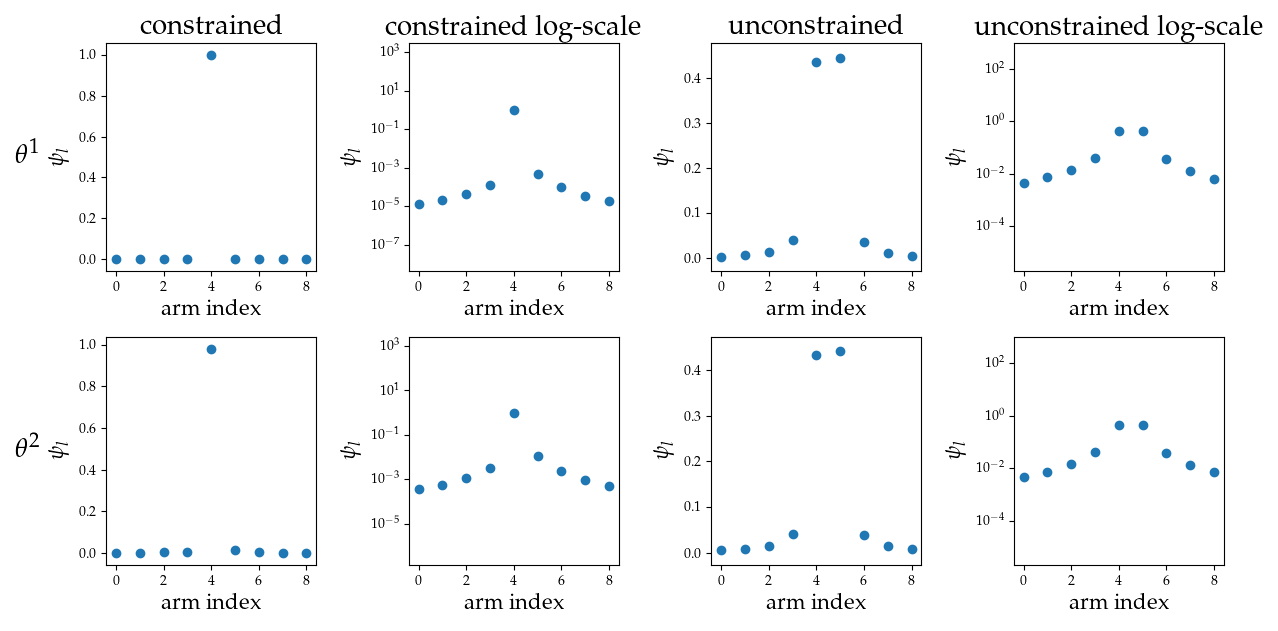
\includegraphics[width=\textwidth]{optimal_allocation.png}
  \caption{Unconstrained and constrained optimal allocation for $\theta_1$ and $\theta_2$, top-4}
  \label{fig:optimal_allocation}
\end{figure}

\section{A sufficient condition for
    optimality}\label{section:optimality_sufficient_condition}
This sufficient condition for convergence towards the optimal allocation is
centered around observing consequences of overallocation. Note that whenever an
allocation is different from the optimal allocation, this implies both over- and
underallocation. We focus on the statement for overallocation, yet an analogous
statement for underallocation should be possible.

In particular, the statement expresses that if an arm $l$ has been
over-allocated so far, indicated by a $\bar{\psi}_{n, l}$ larger than
$\psi^{\frac{1}{2}*}_l$, this over-allocation will be corrected. In this case,
correction means that its likelihood of being sampled in the next and round,
$\psi_{n, l}$ is very low. The intuition of the whole statement being that if
all overallocation is corrected for, then consequently all underallocation is
corrected for as well, by the fact that $\psi$ is a probability distribution.
\begin{proposition}\label{proposition:optimality_sufficient_condition}
  If
  \begin{align}
    \forall l \in [k], \delta > 0: \sum_{n \in \mathbb{N}} \psi_{n, l}
        \mathbb{I}[\bar{\psi}_{n, l} \geq \psi^*_l + \delta] < \infty
        \label{eq:sufficient_condition}
  \end{align}
  then $\bar{\psi}_{n} \rightarrow \psi^*$.
\end{proposition}

\section{Proofs}\label{section:optimal_proofs}
\begin{proof}[\Cref{lemma:set_relation_S*_i}]
  We first show the relationship between $\Theta_{S^*}^c$ and sets
  $\bar{\Theta}_i$ and then show the relationship between $\Theta_{S^*}^c$ and
  $\Theta_{m, j}$.
  \begin{align}
    \Theta_{S^*}^c &= \{\theta \in \Theta | \min_{j \in S^*} \theta_j > \max_{i
        \notin S^*} \theta_i \}^c \\
    &= \{\theta \in \Theta | \max_{i \notin S^*} \theta_i \geq \min_{j \in S^*}
        \theta_j\} \\
    &= \{\theta \in \Theta | \exists i \notin S^*: \theta_i \geq \min_{j \in
        S^*} \theta_j\} \\
    &= \{\theta \in \Theta | \exists i \notin S^*: \text{top-}m(\theta, S^*
        \cup \{i\}) \neq S^*\} \\
    &= \bigcup_{i \notin S^*} \{\theta \in \Theta | \text{top-}m(\theta, S^*
        \cup \{i\}) \neq S^*\} \\
    &= \bigcup_{i \notin S^*} \bar{\Theta}_i \\
    \Theta_{S^*} &= \{\theta \in \Theta | \min_{j \in S^*} \theta_j > \max_{i
        \notin S^*} \theta_i\} \\
    &= \{\theta \in \Theta | \bigwedge_{j \in S^*} \theta_j > \max_{i \notin
        S^*} \theta_i\} \\
    &= \bigcap_{j \in S^*} \{\theta \in \Theta | \theta_j > \max_{i \notin S^*}
        \theta_i\} \\
    &= \bigcap_{j \in S^*} \{\theta \in \Theta | j \in \text{top-}m(\theta,
        [k])\} \\
    &= \bigcap_{j \in S^*} \Theta_{m, j} \\
    \Theta_{S^*}^c &= \Theta - \Theta_{S^*}\\
      &= \Theta - \bigcap_{j \in S^*} \Theta_{m, j}
  \end{align}
\end{proof}

\begin{proof}[\Cref{lemma:posterior_S*_i}]
  First, we prove the equality for $i \notin S^*$, followed by the equality for
  $j \in S^*$.

  The union from \Cref{lemma:set_relation_S*_i} has an additive effect with
  respect to the probability distribution $\Pi_n$. There are $k-m$ possible $i$s
  and each single one leads to a set, whose density is bounded by the maximal
  density of all such sets. This gives us:
  \begin{align}
    \max_{i \notin S^*} \Pi_n(\bar{\Theta}_i) \leq \Pi_n(\Theta_{S^*}^c) \leq (k-m) \max_{i \notin S^*} \Pi_n(\bar{\Theta}_i)
  \end{align}
  We use the definition of $\deq$ to compare lower bound and upper bound.
  \begin{align}
    \lim_{n \rightarrow \infty} \frac{1}{n} \log{\frac{\max_{i \notin S^*} \Pi_n(\bar{\Theta}_i)}{(k-m)\max_{i \notin S^*} \Pi_n(\bar{\Theta}_i)}}
    = \lim_{n \rightarrow \infty} \frac{1}{n} \log{\frac{1}{k-m}} \rightarrow 0
  \end{align}
  Thanks to the lower and upper bound being 'equal' in the $\deq$ sense, we can
  apply the Squeeze theorem\footnote{Also referred to as Sandwich teorem}. We
  obtain the desired result:
  \begin{align}
    \Pi_n(\Theta_{S^*}^c) \deq \max_{i \notin S^*} \Pi_n(\bar{\Theta}_i)
  \end{align}
  For $j \in S^*$, we follow a very similary path by first leveraging the set
  equality from \Cref{lemma:set_relation_S*_i}. Instead of a union, as was the
  case for $i \in S^*$, we are now confronted with an intersection. This implies
  a multiplicative effect on the distribution $\Pi_n$ instead of an additive
  one.
  \begin{align}
    &1 - \min_{j \in S^*} \Pi(\Theta_{m, j}) \leq \Pi(\Theta_{S^*}^c) \leq 1 - \min_{j \in S^*} (\Pi(\Theta_{m, j}))^m \\
  \end{align}
  Again, we will compare upper and lower bound in the $\deq$ sense.
  \begin{align}
    &\lim_{n \rightarrow \infty} \frac{1}{n} \log(\frac{\min_{j \in S^*} \Pi(\Theta_{m, j})}{\min_{j \in S^*} (\Pi(\Theta_{m, j}))^m}) = \lim_{n \rightarrow \infty} \frac{-(m - 1)}{n} \log(\min_{j \in S^*} \Pi(\Theta_{m, j}))
  \end{align}
  Observe that $1 \geq \min_{j \in S^*} \Pi(\Theta_{m, j}) \geq \alpha_{n, S^*} \rightarrow 1$. Hence the limit of the fraction goes to 0 and we have $\min_{j \in S^*} \Pi(\Theta_{m, j}) \deq \min_{j \in S^*} (\Pi(\Theta_{m, j}))^m$. Again, by the Squeeze theorem it follows that
  \begin{align}
    \Pi_n(\Theta_{S^*}^c) \deq 1 - \min_{j \in S^*} \Pi_n(\Theta_{m, j})
  \end{align}
\end{proof}

\begin{proof}[\Cref{lemma:kl_to_C}]
  \begin{align}
    \min_{\theta \in \bar{\Theta}_i} \sum_{j=1}^k \psi_j d(\theta^*_j||\theta_j)
      &= \min_{\theta \in \bar{\Theta}_i} \sum_{j\in S^*}
          \psi_{j}d(\theta^*_{j} || \theta_{j}) + \psi_{i}d(\theta_{i}^* ||
          \theta_{i}) + \sum_{j \notin S^* \cup \{i\}} \psi_j
          d(\theta^*_j||\theta_j) \\
      &= \min_{\theta \in \bar{\Theta}_i} \sum_{j\in S^*}
          \psi_{j}d(\theta^*_{j} || \theta_{j}) + \psi_{i}d(\theta_{i}^* ||
          \theta_{i}) \label{eq: l2_1}\\
      &= \min_{j\in S^*} \min_{\theta \in \bar{\Theta}_i}
          \psi_{j}d(\theta^*_{j} || \theta_{j}) + \psi_{i}d(\theta_{i}^* ||
          \theta_{i}) \label{eq: l2_2}\\
      &= \min_{j\in S^*} \min_{\theta \in \bar{\Theta}_i}
          \psi_{j}d(\theta^*_{j} || \theta_{j}) + \psi_{i}d(\theta_{i}^* ||
          \theta_{j}) \label{eq: l2_3}\\
      &= \min_{j\in S^*} \min_{x \in \mathbb{R}} \psi_{j}d(\theta^*_{j} || x) +
          \psi_{i}d(\theta_{i}^* ||x) \label{eq: l2_4}\\
      &= \min_{j \in S^*} C_{j, i}(\psi_j, \psi_i)
  \end{align}
  \eqref{eq: l2_1} follows from the fact that for any feasible $\theta$, we can
  define an alternative $\theta'$ s.t. $\theta'_i = \theta_i$, $\theta'_j =
  \theta_j$ for all $j \in S^*$ and $\theta'_{i_x} = \theta^*_{i_x}$ for all
  $i_x \notin S^* \cup \{i\}$. For such a $\theta'$, all terms involving $i_x
  \notin S^* \cup \{i\}$ are zero by the definition of the KL divergence while
  all others terms remain unchanged. Hence the minimum occurs with such a
  $\theta'$. Importantly, $\theta'$ remains feasible according to current
  definitions of $\bar{\Theta}_i$, i.e. $\theta' \in \bar{\Theta}_i$.

  \eqref{eq: l2_2} follows from a similar observation: only a single arm from
  $S^*$ needs to be inferior to arm $i$ under $\theta$. Recall that the terms of
  the individual arms do not influence each other. This implies that the
  minimization will gravitate towards setting all but one arm from $S^*$ in
  $\theta$ to the their true value - as the KL divergence is minimized for the
  true values. Hence the terms of all but one arm from $S^*$ will be cancelled
  out by the minimization. As $i$ remains superior to one arm in $S^*$, we have
  top-$m(\theta, S^* \cup \{i\}) \neq S^*$. Thereby such a $\theta$ is feasible
  according to $\bar{\Theta}_i$.

  \eqref{eq: l2_3} follows from monotonicity of the KL divergence, as displayed
  in \Cref{eq:kl_monotonicity}, combined with the possibility of $\theta_i =
  \theta_j$ tells us that the minimum will be reached in the case of equality.

  \eqref{eq: l2_4} follows from observing that our minimization over $\theta$
  has reduced to a minimization over $\theta_j$. The latter is a one-dimensional
  real as we are in the case of distributions belonging to the one-dimensional exponential family.
\end{proof}

\begin{proof}[\Cref{lemma:C_concave}]
  For the sake of clarity, let us define
  \begin{align}
    f(x, (\psi_j, \psi_i)) = \psi_j d(\theta_j^*||x) + \psi_i d(\theta_i^* || x)
  \end{align}
  Note that $C_{j, i}(\psi_j, \psi_i) = min_{x \in \mathbb{R}} f(x,(\psi_j, \psi_i))$. Clearly, $f$ is linear in $(\psi_j, \psi_i)$. According to Boyd and Vandenberghe (3.2.5) \cite{Boyd:2004:CO:993483}, the minimum over a family of linear functions is concave.
\end{proof}

\textbf{\Cref{lemma:C_unique_solution}}
Assume $A'(\theta)$ to be the mean observation under $\theta$. Given a $j \in S^*$, the solution to the minimization problem \eqref{eq:C} in $x$ is $\bar{\theta} \in \mathbb{R}$, satisfying:
\begin{align}
  A'(\bar{\theta}) = \frac{\psi_j A'(\theta_j^*) + \psi_i
      A'(\theta_i^*)}{\psi_j + \psi_i}
\end{align}
Therefore
\begin{align}
  C_{j, i}(\psi_j, \psi_i) = \psi_j d(\theta^*_j || \bar{\theta}) + \psi_i
      d(\theta^*_i || \bar{\theta})
\end{align}
\begin{proof}[\Cref{lemma:C_unique_solution}]
  By \Cref{eq:exponential_kl} we know that for the exponential family of probability distributions it holds that:
  \[d(\theta||\theta') = (\theta - \theta')A'(\theta) - A(\theta) + A(\theta')\]
  Applying this identity to the definition of $C_{j, i}$ \label{eq:C} for given $j$, $i$, $\psi_j$, $\psi_i$ gives us:
  \begin{align}
    &\psi_{j}d(\theta^*_{j} || x) + \psi_{i}d(\theta_{i}^* ||x) \\
    &=\psi_j ((\theta_j^* - x)A'(\theta_j^*) - A(\theta_j^*) + A(x)) + \psi_i((\theta_i^* - x)A'(\theta_i^*) - A(\theta_i^*) + A(x))\\
    &= -x(\psi_j A'(\theta_j^*) + \psi_i A'(\theta_i^*)) + A(x)(\psi_j + \psi_i) + c
  \end{align}
  Where $c$ is independent of $x$. As we seeks to minimize this quantity with respect to $x$, we differentiate it with respect to $x$ and set it to 0. This yields:
  \[A'(x) = \frac{\psi_j A'(\theta_j^*) + \psi_i A'(\theta_i^*)}{\psi_j + \psi_i}\]
\end{proof}

\begin{proof}[\Cref{lemma:C_strictly_increasing}]
  We will proceed to show for fixed $j \in S^*$ and $i \notin S^*$, $C_{j, i}$
  is increasing in its first argument $\psi_j$ as its second argument $\psi_i$
  follows by symmetry.

  Let us define $f(x, \psi_j, p) = \psi_j d(\theta_j^*||x) + p d(\theta_i^*||x)$
  which implies that $C_{j, i}(\psi_j, p) = \min_{x \in \mathbb{R}} f(x, \psi_j,
  p)$. We first show that $f$ is strictly increasing in $\psi_j$ and will use
  that to show that the initial claim.

  As the KL divergence is non-negative we have:
  \begin{align}
    f(x, \psi_j + \epsilon, p) &= \psi_j d(\theta_j^*||x) + \epsilon
        d(\theta_j^*||x) + p d(\theta_i^*||x) \\
      &> p d(\theta_i^*||x) + \psi_j d(\theta_j^*||x)\\
      &= f(x, \psi_j, p)
  \end{align}
  And therefore $f$ is strictly increasing in $\psi_j$.

  For a given $p$, we fix $\psi_{j1} < \psi_{j2}$ from $[0, 1]$ as well as their counterparts
  \begin{align}
    &x_1 = \argmin_{x \in \mathbb{R}} f(x, \psi_{j1}, p)
    &x_2 = \argmin_{x \in \mathbb{R}} f(x, \psi_{j2}, p)
  \end{align}
  Hence our goal is to show that $f(x_1, \psi_{j1}, p) < f(x_2, \psi_{j2}, p)$.
  By \Cref{lemma:C_unique_solution} both $x_1$ and $x_2$ are unique. Hence
  \begin{align}
    f(x_1, \psi_{j1}, \alpha) &< f(x_2, \psi_{j1}, \alpha) \\
    f(x_2, \psi_{j2}, \alpha) &< f(x_1, \psi_{j2}, \alpha)
  \end{align}
  As $f$ is strictly increasing in its second argument, it holds that $f(x_2,
  \psi_{j1}, \alpha) < f(x_2, \psi_{j2}, \alpha)$. Chaining those inequalities
  together we obtain:
  \begin{align}
    f(x_1, \psi_{j1}, \alpha) < f(x_2, \psi_{j1})  < f(x_2, \psi_{j2}) < f(x_1,
        \psi_{j2})
  \end{align}
\end{proof}

\begin{proof}[\Cref{proposition:characterization}]
  We prove in the following order: \eqref{itm:p7_i} \eqref{eq:condition_C} must
  hold for an optimal allocation, \eqref{itm:p7_ii} an optimal allocation is
  unique. After this, the remaining claim, namely that no other constrained
  allocation can be better, follows directly.
  \begin{enumerate}[(i)]
    \item \label{itm:p7_i} Suppose that $\psi^{\frac{1}{2}*}$ is optimal but does not satisfy \eqref{eq:condition_C}. Hence for some $i_1, i_2 \notin S^*, j_1, j_2 \in S^*$ with $(j_1, i_1) \neq (j_2, i_2)$:
    \[C_{j_1, i_1}(\psi^{\frac{1}{2}*}_{j_1}, \psi^{\frac{1}{2}*}_{i_1}) > C_{j_2, i_2}(\psi^{\frac{1}{2}*}_{j_2}, \psi^{\frac{1}{2}*}_{i_2})\]
    This implies:
    \[C_{j_1, i_1}(\psi^{\frac{1}{2}*}_{j_1}, \psi^{\frac{1}{2}*}_{i_1}) > \min_{i \notin S^*} \min_{j \in S^*}C_{j, i}(\psi^{\frac{1}{2}*}_j, \psi^{\frac{1}{2}*}_i) \]
    Consider the the measurement plan $\psi^\epsilon$ with
    \begin{itemize}
      \item $\psi^\epsilon_{i_1} = \psi^{\frac{1}{2}*}_{i_1} - \epsilon$
      \item $\psi^\epsilon_{j_1} = \psi^{\frac{1}{2}*}_{j_1} - \epsilon$
      \item $\forall l\notin \{i_1, j_1\}: \psi^\epsilon_l = \psi^{\frac{1}{2}*}_\gamma + \frac{2 \epsilon}{k-2}$
    \end{itemize}
    We can choose $\epsilon$ sufficiently small such that we preserve the inequality
    \begin{align}
      C_{j_1, i_1}(\psi^\epsilon_{j_1}, \psi^\epsilon_{i_1}) > C_{j_2, i_2}(\psi^\epsilon_{j_2}, \psi^\epsilon_{i_2})
    \end{align}
    while shifting enough measurement to all other arms such that
    \begin{align}
      \min_{i \notin S^*} \min_{j \in S^*} C_{j, i}(\psi^\epsilon_{j}, \psi^\epsilon_i) > \min_{i \notin S^*} \min_{j \in S^*} C_{j, i}(\psi^{\frac{1}{2}*}_j, \psi^{\frac{1}{2}*}_i)
    \end{align}
    Hence $\psi^\epsilon$ obtains more evidence on the worst possible pair than
    $\psi^{\frac{1}{2}*}$ and thereby achieves a better convergence rate
    \eqref{eq:constrained_optimal_gamma}. In other words, $\psi^{\frac{1}{2}*}$
    is not optimal, which is a contradiction.

    \item \label{itm:p7_ii} Suppose that there are optimal $\psi^1$, $\psi^2$,
    therefore both satisfying \eqref{eq:condition_C} with the exact same value
    $C^*$. It follows that there is at least one $l$ s.t. $\psi^1_{l} \neq
    \psi^2_{l}$. W.l.o.g. assume $l = i_x \notin S^*$ and $\psi^1_{i_x} >
    \psi^2_{i_x}$.

    We proceed by case distinction and show that each leads to a contradiction.
    \begin{itemize}
      \item Only one arm is disinct.

      For some $\epsilon > 0$ and any $j \in S^*$ have
      \begin{align}
        C_{j, i_x}(\psi^2_j, \psi^2_{i_x} + \epsilon) &= C_{j, i_x}(\psi^1_j, \psi^2_{i_x} + \epsilon) \\
        &= C_{j, i_x}(\psi^1_j, \psi^1_{i_x}) \\
        &= C^* \\
        &= C_{j, i_x}(\psi^2_j, \psi^2_{i_x})
      \end{align}
      Which is a contradiction as $\epsilon$ is positive $C_{j, i_x}$ strictly increasing by \Cref{lemma:C_strictly_increasing}.
      \item More that one arm is distinct, but they all belong to either $S^*$ or $S^{*c}$.

      As our distinct value so far comes from $S^{*c}$, let's also assume, w.l.o.g., $i_y \notin S^*$ with $i_y \neq i_x$.

      Note that independently of whether $\psi^1_{i_y} \geq \psi^2_{i_y}$ or $\psi^1_{i_y} < \psi^2_{i_y}$ holds, the previous argument can be applied for any $j \in S^*$.

      \item At least one arm is distinct in both $S^*$ and $S^{*c}$.

      Let's assume first that the distinctive optimal arm is $j_x \in S^*$.
      Observe that $\psi^1_{j_x} < \psi^2_{j_x}$ has to hold, otherwise both
      $i_x$ and $j_x$ were allocated more weight in $\psi^1$ than in $\psi^2$.
      By \Cref{lemma:C_strictly_increasing} we recall the increase of $C_{j_x,
      i_x}$ in both of its arguments. This implies greater evidence for $\psi^1$
      than for $\psi^2$, a contradiction to the assumption that both are
      optimal.

      Recall our constraint $\frac{1}{2} = \sum_{j \in S^*} \psi_l = \sum_{i \notin S^*} \psi_i$, which has to hold for both $\psi^1$ and $\psi^2$.
      Hence for $psi^1$'s over-allocation on $i_x$, there has to be an $i_y \notin S^*$ for which $\psi^1$ underallocates, compared to $psi^2$.
      Summarizing, we have:
      \begin{itemize}
        \item $\psi^1_{i_x} = \psi^2_{i_x} + \epsilon$
        \item $\psi^1_{j_x} = \psi^2_{j_x} - \epsilon'$
        \item $\psi^1_{i_y} = \psi^2_{i_y} - \epsilon''$
      \end{itemize}
      Combining this with the fact that all $C$ values from both $\psi^1$ and $\psi^2$ have to equal one another, we obtain:
      \begin{align}
        C_{j_x, i_y}(\psi^2_{j_x} - \epsilon', \psi^2_{i_y} - \epsilon'') &= C_{j_x, i_y}(\psi^1_{j_x}, \psi^1_{i_y}) \\
        &= C^* \\
        &= C_{j_x, i_y}(\psi^2_{j_x}, \psi^2_{i_y})
      \end{align}
      which, again, is a contradiction by the strictly increasing nature of $C_{j_x, i_y}$.
    \end{itemize}
  \end{enumerate}
\end{proof}

\begin{proof}[\Cref{proposition:optimality_sufficient_condition}]
  First, we prove that $\liminf_{n \rightarrow \infty} \bar{\psi}_{n, l} \leq \psi^*_l$ by contradiction.
  Assume otherwise. Then there are $n_0$ and $\delta$ such that for all $n > n_0:$ $\bar{\psi}_{n, l} \geq \psi^*_l + \delta$.
  \begin{align}
  \sum_{n \in \mathbb{N}} \psi_{n, i} &= \sum_{n \in [0, n_0]} \psi_{n, l} + \sum_{n \in [n_0 + 1, \infty]} \psi_{n, l} \\
  &= \sum_{n \in [0, n_0]} \psi_{n, l} +  \sum_{n \in [n_0 + 1, \infty]} \psi_{n, l}\mathbb{I}[\bar{\psi}_{n, l} \geq \psi^*_l + \delta]
  \end{align}
  The first term is finite as it consists of finitely many terms that are each finite themselves, in particular bounded from above by 1. The second term is finite by the assumption of the Lemma and the knowledge that $\psi$ is positive. Hence $\sum_{n \in \mathbb{N}} \psi_{n, l} < \infty$.
  \begin{align}
  \lim_{n \rightarrow \infty} \sum_{l \in [k]} \bar{\psi}_{n, l} = \lim_{n \rightarrow \infty} \sum_{l \in [k]} \frac{\sum_{n' \in [n]} \psi_{n', l}}{n} \rightarrow 0
  \end{align}
  However, we know by the definition of $\psi$ that for any $n$, $\sum_{n' \in [n]} \sum_{l \in [k]} \bar{\psi}_{n, l}  = n$, which is a contradiction.

  Second, we will prove that $\limsup_{n \rightarrow \infty} \bar{\psi}_{n, l}
  \leq \psi^*_l$ by contradiction. Assume otherwise. Combined with the previous
  point, this implies that for infinitely many $n$, $\bar{\psi}_{n, l}$ is above
  and for infinitely many it is below $\psi^*_l$. As $n$ belongs to a countable
  set, those points below and above have to alternate. This implies that our
  indicator function is 'triggered' infinitely many times. Observe that if
  $\psi_{n, l}$ is 0 once, it will never increase again as no posterior updates
  will be made. Hence every time the indicator function is triggered, $\psi_{n,
  l}$ has to be stricly positive; otherwise $l$ would never be sampled again and
  $\bar{\psi}_{n, l}$ monotonically decrease, even though it oscillates. As a
  consequence, we have an infinite amount of non-zero, positive values and hence
  \[\sum_{n \in \mathbb{N}} \psi_{n, l} \mathbb{I}[\bar{\psi}_{n, l} \geq
      \psi^*_l + \delta] = \infty\]
  which violates the assumption of the lemma and thereby is a contradiction.

  With the help of our initial assumption we know that for all $l$ it holds that
  $\limsup \bar{\psi}_{n, l} \rightarrow \psi^*_l$. This, combined with the fact
  that $\sum_{l \in [k]} \bar{\psi}_{n, l} = \sum_{l \in [k]} \psi^*_{l}$ allows
  us to conclude that $\bar{\psi}_{n} \rightarrow \psi^*$.
\end{proof}
